\documentclass[12pt]{report}   						% list options between brackets
\usepackage{listings}               			% list packages between braces3
\usepackage{xcolor}								% Needed to define custom colors for code
\usepackage{graphicx}											% Needed to embed vector graphics								
\usepackage[parfill]{parskip}							% no identation begining paragraph and empty line between paragraphs
\usepackage{float}												% Needed to place figure exactly
%\usepackage[superscript,biblabel]{cite} 	% Needed to superscript references
\usepackage{epstopdf}
\frenchspacing

\setcounter{secnumdepth}{2}
\setcounter{tocdepth}{2}
\setlength{\belowcaptionskip}{0pt} 				%space after figure text
\setlength{\abovecaptionskip}{5pt} 				%space before figure text

% type user-defined commands here
\lstdefinelanguage{CSharp}
{
 morecomment = [l]{//}, 
 morecomment = [l]{///},
 morecomment = [s]{/*}{*/},
 morestring=[b]", 
 sensitive = true,
 morekeywords = {abstract,  event,  new,  struct,
   as,  explicit,  null,  switch,
   base,  extern,  object,  this,
   bool,  false,  operator,  throw,
   break,  finally,  out,  true,
   byte,  fixed,  override,  try,
   case,  float,  params,  typeof,
   catch,  for,  private,  uint,
   char,  foreach,  protected,  ulong,
   checked,  goto,  public,  unchecked,
   class,  if,  readonly,  unsafe,
   const,  implicit,  ref,  ushort,
   continue,  in,  return,  using,
   decimal,  int,  sbyte,  virtual,
   default,  interface,  sealed,  volatile,
   delegate,  internal,  short,  void,
   do,  is,  sizeof,  while,
   double,  lock,  stackalloc,   
   else,  long,  static,   
   enum,  namespace, string, var, partial}
}

\usepackage{color}
\usepackage{textcomp}
\definecolor{listinggray}{gray}{0.9}
\definecolor{lbcolor}{rgb}{0.95,0.95,0.95}
\lstset{
  % backgroundcolor=\color{lbcolor},
  tabsize=2,
  frame=tb,
  language=CSharp,
  basicstyle=\scriptsize,
  upquote=true,
  aboveskip={1.5\baselineskip},
  columns=fixed,
  showstringspaces=false,
  extendedchars=true,
  breaklines=true,
  % frame=single,
  showtabs=false,
  showspaces=false,
  showstringspaces=false,
  identifierstyle=\ttfamily,
  keywordstyle=[1]\ttfamily\color[rgb]{0,0,1},
  keywordstyle=[2]\ttfamily\color[rgb]{0.1,0.6,0.6},
  commentstyle=\ttfamily\color[rgb]{0.133,0.545,0.133},
  stringstyle=\ttfamily\color[rgb]{1,0,0},
}

\begin{document}

% Front page
\title{Mixed Side C Sharp (MiCS)}
\author{Asger Schlichtkrull \& Tomas Lieberkind}
\date{May 22, 2013}
\maketitle

% Abstract
\begin{abstract}
	To improve development of web applications with ASP.NET Web Forms this report investigates how JavaScript can be safely represented in order to acheive compile time validation. To improve safe development further the report investigates if consistency between client and server side can be guaranteed. Additionally the report investigates if server side code can be ported to client side code, as this would give additional safety and maintenance benefits.

	Developing web applications instead of native applications is a strong tendency in software development today. JavaScript contributes to enriching the user experience and sometimes provides functionality which is indispensable for such web applications.

	JavaScript however, can in many ways be regarded as an unsafe programming language. Because of this many projects (e.g. Microsoft’s TypeScript or Google Web Toolkit) have built safe environments for writing client side scripts to help enforce correctness.


	The report concludes...
\end{abstract}

\tableofcontents


\chapter{Introduction} % (fold)
\label{cha:introduction}
	This bachelor project has been produced by Tomas Alan Lieberkind and Asger Schlichtkrull from the 1st February 2013 to the 22nd May 2013 at the IT-University of Copenhagen. The project has been supervised by Peter Sestoft.

	\section{Motivation} % (fold)
\label{sec:motivation}
	We would like to improve development of web applications with ASP.NET Web Forms and therefore it is beneficial to investigate how JavaScript can be from a .NET language such as C\# or F\# in order to achieve compile time validation. % Todo: synes denne første del er lidt underlig...

	Developing web applications instead of native applications is a strong tendency in software development today. JavaScript contributes to enriching the user experience and sometimes provide functionality which is indispensable for such web applications.

	ASP.NET Web Forms provides the possibility of building HTML documents using C\# which improves correctness through compile time validation. Writing JavaScript code using C\# is not possible in the same way as with HTML documents. JavaScript is embedded into the application as text strings and thus compile time validation is not possible. This increases the possibility of writing faulty scripts that emits errors which are not discovered before client side runtime. Runtime errors are generally harder to debug and in worst case exposed to the end user while leaving the application in a corrupt state.

	Achieving compile time validation of JavaScript is not a ground-breaking thought, and there are several existing projects that do exactly this; TypeScript by Microsoft and Dart by Google are just a few.

	Depending on the situation one weakness with some of these solutions are that the server side code and the client side code is written as two independent units, and nothing ties them safely together. 

	Another problem is that of reusability. In cases such as form validation it is necessary to write the same piece of code in two different languages in order to validate both on client side and server side.

	This project aims to find a solution for safe JavaScript development that; incorporates compile time validation, enables reusability of server side code on client side and tries to ensure consistency between the server side generated Html document and the client side script code.
% section motivation (end)



\section{Reading Guide}

	This report is directed to people with interest in how JavaScript can be safely written in Microsoft ASP.NET web applications. It is assumed that the reader has a general understanding of Abstract Syntax Trees and a basic understanding of JavaScript. Third party libraries used in the project, namely Roslyn and Script\#, will be introduced and thus knowledge about these is not a prerequisite.

	This report proposes a solution where JavaScript is written safely by translating C\# to JavaScript. This approach makes it possible to execute the same code both on server and client side and is therefore called Mixed Side C Sharp (MiCS).

	This document consists of nine chapters.

	Chapter one introduces the project, the motivation behind it and its scope. Additionally it introduces the case study upon which it is based.

	Chapter two briefly introduces Microsoft ASP.NET Web Forms and the usage of Code Behind to develop web applications. Furthermore it explains why JavaScript can be considered an unsafe language.

	Chapter three introduces various technologies that can be useful to the project and describes how they can be used in combination to approach the problem definition in different ways. Furthermore an analysis is conducted in order to investigate which approach is most convenient to implement. The chosen solution is called MiCS.

	Chapter four is a short manual that describes how MiCS is used.

	Chapter five describes the MiCS project main workflow, architecture and other design decisions.

	Chapter six describes the implementation of MiCS; how types are handled and mapped, validation of mixed and client side code, mapping of ASTs and script generation.

	Chapter seven shortly describes the testing done in the MiCS project.
	
	Chapter eight evaluates the MiCS solution, reflects on the design goals set in the problem definition and discusses what future directions the project could take from here.

	Chapter nine is the report conclusion.

	In the report we use the terms developer and end user. The developer is a person that uses MiCS to write mixed side and client side code. The end user is the person that use the web application created by the developer.
	% Todo: Update reading guide as one the last things...
	% Todo: Introduce DOM, Safety vs security, when we say JavaScript we JavaScript in the browser
	% Todo: The read should have knowledge of DSL, JavaScript (script), client server side, DOM


\section{Problem definition}
	The problem definition has changed since the beginning of this project. Originally we wanted to represent JavaScript as an internal DSL in C\#. Instead we widened our perspective, to include other possible approaches to safe JavaScript development in ASP.NET Web Forms. Below, the revised problem definition is listed.
	\begin{itemize}

	\item Study JavaScript and describe its unsafe language features.

	\item Investigate how JavaScript can be generated from C\# or F\#.
	\item Investigate how correct interaction between JavaScript and Html elements can be guaranteed.

	\item Investigate how to implement a solution that generates JavaScript from server side code (client-server side portability).

	\item Implement and test a class library that supports safe JavaScript development from Code Behind.


	\end{itemize}

	\subsection{Learning goals}
		\begin{itemize}

		\item Better knowledge of JavaScript in general and the more subtle language features of the language.
		\item Better knowledge of ASP.NET Web Forms.
	 	\item Better understanding of the difference between C\#/.NET (as a static typed) language and JavaScript (dynamically typed language).
		\item Better understanding of web development and the communication between client and server side...
		\item Basic knowledge of cross compilers and abstract syntax trees.
		\end{itemize}

\section{Method}
	\begin{itemize}
	\item We will study JavaScript literature to obtain a better understanding JavaScript and which of its features can be considered unsafe. 
	\item We will investigate what technologies and libraries can contribute to the project and how these combined can be used to approach solutions in different ways.
	\item We will analyse and compare the solutions in order to find the one that best fits this project
	\item We will design and implement the solution from step 2.
	\item We will set up a unit test suite in order to ensure that everything works as expected.
	\end{itemize}

\section{Scope}
	% Todo: Do we say something about the use of DOM types is down prioritized?
	% Todo: Only JavaScript in the browser.
	Mapping the entire C\# language to JavaScript is unrealistic given the time constraints on this project. Only the subset of C\# needed to fulfill the requirements set by the case study will be taken into account.

	\subsection{Case Study}
		A common use case of JavaScript is form validation. As a user experience enriching feature, forms are often validated on client side, as to avoid the waiting time for a page load. However, forms have to be validated on the server side as well since the client side validation is easily bypassed. Our case study concerns the validation of a registration form. Specifically, we would like to be able to:

		\begin{itemize}
			\item Validate strings using Regular Expressions to check if email addresses, postal addresses and phone numbers are correctly formatted
			\item Validate the length of strings to check that users do not enter an exceptionally long string, e.g. as their name
			\item Validate dependencies between input (conditional logic). E.g. validation of a text field depends on whether or not a check box is checked.
		\end{itemize}

		Figure~\ref{registrationForm} shows the registration form, and below, the validation criteria are explained.

		\begin{figure}
			\begin{center}
				\centerline{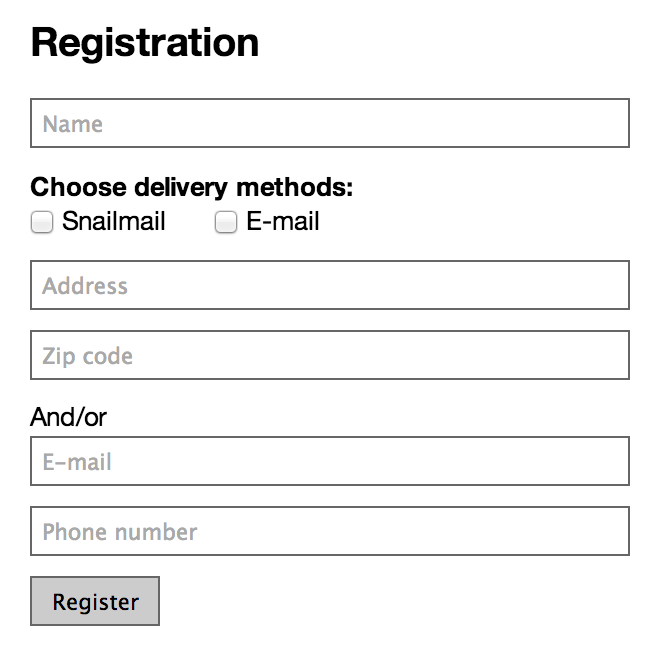
\includegraphics[width=7cm]{resources/images/registrationform.png}}
			\end{center}
			\caption{The form that we aim at validating}
			\label{registrationForm}
		\end{figure}

		\begin{itemize}
			\item The name has to consist of at least a first name and a last name, cannot be less than 5 characters long and not exceed 128 characters
			\item At least one delivery method has to be checked. If “Snailmail” is checked, the address and zip code fields have to be filled in. If “E-mail” is checked, the “E-mail” field has to be filled in.
			\item The address has to follow the format: \newline\newline \texttt{(streetname) (house number)[, (floor number). (TH|TV|SAL)]}\newline\newline where everything within the brackets is optional. For example, the addresses ``Amagerbrogade 125, 3.TV'' and ``Englodden 4'' are valid addresses whereas ``Griffenfeldsgade'' and ``Svinget 34, 4'' are not.
			\item The zip code has to consist of four integer characters (Danish zip code).
			\item The e-mail has to be a valid e-mail
			\item The phone number has to consist of 8 numbers, where the first number cannot be “0”.
		\end{itemize}


	\subsection{Safety Considerations} % (fold)
	\label{sub:safety_considerations}
		This section will address some fundamental aspects of safe development that we would like to target in this project.
		% There are some fundamental aspects of safe development that we will like to target in this project and which we will describe here. 

		\subsubsection{Compile Time Errors vs. Runtime Errors} % (fold)
		\label{ssub:compile_time_errors_vs_runtime_errors}
			
			When considering web applications, errors can occur both on server side and client side. On server side, errors can occur on either compile time or runtime. On client side, compile time does not exist, and consequently errors can only occur on runtime.
			Compile time errors are generally easier to debug than runtime errors and thus fixing them is often less time consuming. Client side runtime errors will be exposed to web application's end users which is highly undesirable. Because of this, one of the fundamental goals of MiCS is to move errors from client side runtime to server side (runtime or compile time, see Figure \ref{movingErrors}).

			\begin{figure}
				\begin{center}
					\centerline{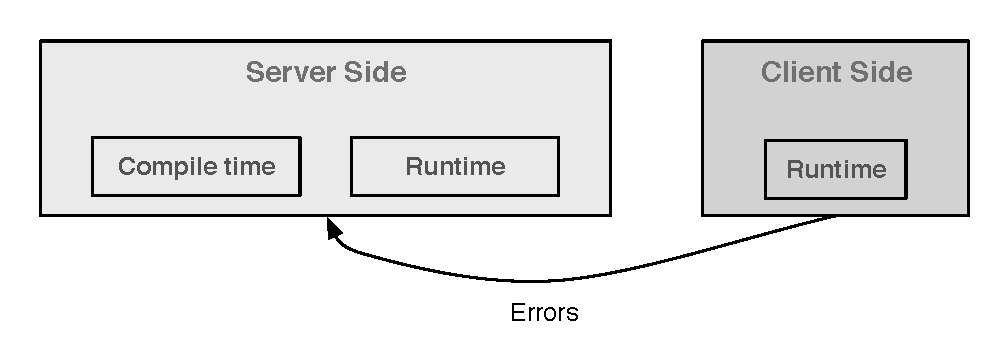
\includegraphics[width=11cm]{resources/images/MovingErrors.eps}}
				\end{center}
				\caption{Improving safe development by trying to move errors from client side to server side.}
				\label{movingErrors}
			\end{figure}
		% subsubsection compile_time_errors_vs_runtime_errors (end)

		\subsubsection{JavaScript DOM Consistency} % (fold)
		\label{ssub:javascript_dom_consistency}
			When building a web page a typical setup is a document consisting of Html elements (DOM elements) and some client side JavaScript. The client side scripts then modifies the Html elements in response to user interactions. There are however no guarantee of correct interaction between the JavaScript and the Html elements. E.g. when calling a JavaScript function from a button \texttt{onclick} event it is possible to have misspelled the function name which would cause a client side error.

			In the context of safe JavaScript development in the browser this can be considered a somewhat critical issue. Therefore a compile time guarantee of the consistency between JavaScript code and DOM elements (or vice versa) would be an improvement.

		% subsubsection server_client_consistency (end)

	% subsection safety_considerations (end)

	\subsection{Focus} % (fold)
	\label{sub:focus}
		This project primarily serves as a proof-of-concept and therefore the main focus will be to generate code that actually works, and can fulfill the requirements set by the case study. 

		This project will only be considering solutions that can be use with Microsoft’s ASP.NET Web Forms. Furthermore the solution has to be utilized using C\#.

		The quality of the generated JavaScript will not be assessed. The primary reason for this is that the JavaScript will be generated by reusing parts of the Script\# framework in the solution we suggest in this project.

		Likewise overall performance will not be analyzed because of time constraints on the project.
	% subsection focus (end)


\section{Target Audience} % (fold)
\label{sec:section_name}
	The target audience is developers who create web applications using ASP.NET Web Forms with C\# where correctness is of high priority. This implies that the developer aims at displaying a 100\% working web application or nothing at all. An error message is preferred over an application in a corrupt, or partly corrupt, state.
% section section_name (end)


% chapter introduction (end)





\chapter{Background}

\section{ASP.NET Web Forms} % (fold)
\label{sec:asp_net_web_forms}
	% Todo: explain Active Server Pages
	ASP.NET. Web Forms are the User Interface (UI) elements that give your Web applications their look and feel. Web Forms are similar to Windows Forms \cite{msdn01} in that they provide properties, methods, and events for the controls that are placed onto them. However, these UI elements render themselves into Html \cite{msdn02}. When working with Web Forms you can both write markup code and write C\# code from Code Behind (explained in \ref{sub:code_behind}) when building a web application. 

	\begin{figure}[H]
					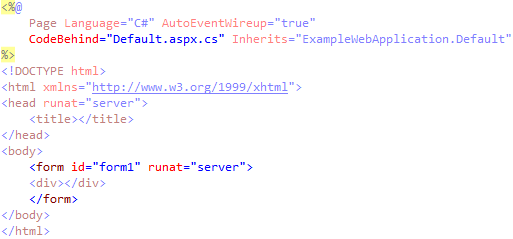
\includegraphics[width=8cm]{resources/images/Markup.png}
				\caption{Markup code in Default.aspx}
				\label{markup}
			\end{figure}

	\subsection{Code Behind} % (fold)
	\label{sub:code_behind}
		The web page Default.aspx is associated to a C\# file, Default.aspx.cs, where the page has different events that can be utilized. This is \texttt{Default.aspx}'s \emph{Code Behind} file. In figure \ref{codeBehind} a button control is added to the form \texttt{form1} (defined in markup in figure \ref{markup}) via the page’s Load event. This is opposed to adding the button in markup code.


				\begin{figure}
					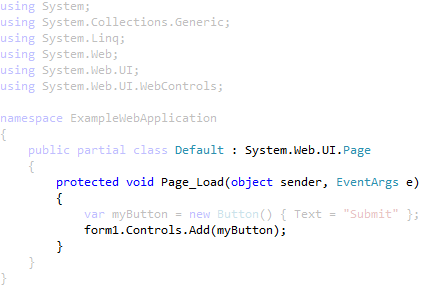
\includegraphics[width=10cm]{resources/images/CodeBehind.png}
				\caption{Default.aspx.cs Code Behind file associated to the Default.aspx page.}
				\label{codeBehind}
			\end{figure}
		The resulting web page and source will be as shown in figure \ref{html} (with Chrome Development Tools).

				\begin{figure}
					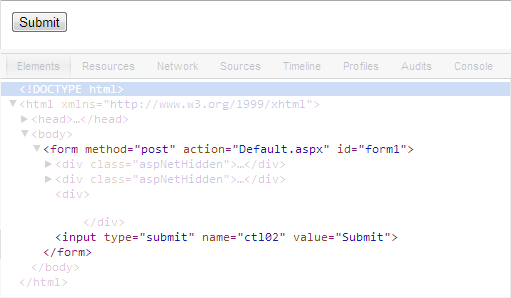
\includegraphics[width=12cm]{resources/images/Html.png}
				\caption{Resulting web page and source code of the Default.aspx page.}
				\label{html}
			\end{figure}
		There are built-in control classes equivalent to most DOM elements so in this manner one can build an entire web application from Code Behind. Some of the benefits of working from Code Behind is that you essentially achieve compile time validation of your markup code and you get to work in object oriented manner.

		todo: Web Forms unsafe JavaScript example.
	% subsection code_behind (end)

% section asp_net_web_forms (end)

\section{JavaScript and its Unsafe Language Features} % (fold)
\label{sec:javascript_and_its_unsafe_language_feature}
	
	JavaScript is an interpreted, dynamically typed scripting language used mainly for making web applications with dynamic user interfaces. JavaScript inherits its syntax from C, and was developed by Netscape in 1995 \cite{bib:wiki_javascript}. Today, JavaScript is used in almost all big web applications, but despite its popularity, it has some language features that can be considered unsafe when correctness is of high priority. The remainder of this section will highlight some of these unsafe language features.

	\subsection{No compile time validation} % (fold)
	\label{sub:no_compile_time_validation}
		In general enforcing correctness at compile time instead of runtime makes the development process safer as some errors (e.g.\ syntax errors like missing semicolons) are not possible to overlook or ignore. Furthermore discovering errors as early as possible makes the debugging process easier hence compile time errors should be preferred over runtime errors. So the fact that JavaScript is an interpreted language that is not compiled makes it a less safe language.
	% subsection no_compile_time_validation (end)

	\subsection{Dynamic type system} % (fold)
	\label{sub:dynamic_type_system}
		JavaScript has a dynamic type system which in some situations make the development process faster but also less safe as some errors will not emerge at all (or maybe emerge at runtime). E.g. it is possible to by mistake add a Number value with a Boolean value without getting any warnings. In other words it is possible to forget enforcing that a variable has a specific type. This problem is amplified when parsing external input as it is done e.g.\ in form validation.
	% subsection dynamic_type_system (end)

	\subsection{Reuse of identifiers in declarations} % (fold)
	\label{sec:reuse_of_identifiers_in_declarations}
		JavaScript allows declaring multiple variables or functions with the same name in the same execution context without any warnings. This makes it possible by mistake to override earlier declared variables or functions. This kind of errors can be difficult and time consuming to discover because of their hidden nature.
	% section reuse_of_identifiers_in_declarations (end)

	\subsection{No block scope} % (fold)
	\label{sub:no_block_scope}
		JavaScript's syntax comes from C. In all other C-like languages a block creates scope. This is not the case in JavaScript even though its block syntax suggests that it does (“The Good Parts” p. 102). This can be a source of confusion especially for programmers that are used to block scope. Scope related errors might be difficult to debug as obviously no warnings are given (since there is no block scope) when a variable from an outer block is assigned a value by mistake.
	% subsection no_block_scope (end)

	\subsection{Implicit Type Conversion} % (fold)
	\label{sub:implicit_type_conversion}
	TODO
	% subsection implicit_type_conversion (end)

	\subsection{Many ''falsy'' values} % (fold)
	\label{sub:many_falsy_values}
		TODO: Clarify this
		JavaScript has multiple falsy values which are not interchangeable. This is another source of errors that can be difficult to discover (“The Good Parts” p. 106).
	% subsection many_falsy_values (end)
% section javascript_and_its_unsafe_language_feature (end)

\section{Related works} % (fold)
\label{sec:related_works}
TODO
% section related_works (end)


\chapter{Approach Analysis}
	As mentioned in the Problem Definition, it was decided to conduct an analysis in order to find out which approach would best fit this project. This chapter will give an overview of different technologies we have considered to use and describe how they can be used in combination to approach the project in different ways. Lastly, a comparison of the approaches will be made, in order to decide on which approach to implement.

\section{Technologies}
	In this section we will give a brief description of the technologies associated to the different approaches we have considered.

	\subsection{Script\#} % (fold)
	\label{sub:subsection_name}
		Script\# \cite{scriptsharp} is a cross-compiler from C\# to JavaScript that is maintained by Nikhil Kothari \cite{nikhilk} from Microsoft. The way ScriptSharp works is that it compiles an entire C\# project to client side JavaScript code.

		The main assembly ScriptSharp.dll is shown in figure \ref{simplifiedOverview} as a simplified dependency diagram with the most relevant assemblies related to our project. When Script\# is used in a regular manner a C\# AST is built from the C\# source code using classes from the Parser and CodeModel namespaces. The ScriptModel namespace contains classes for building the JavaScript AST before the actual script is generated using classes in the Generator namespace.

		\begin{figure}[H]
			\begin{center}
				\centerline{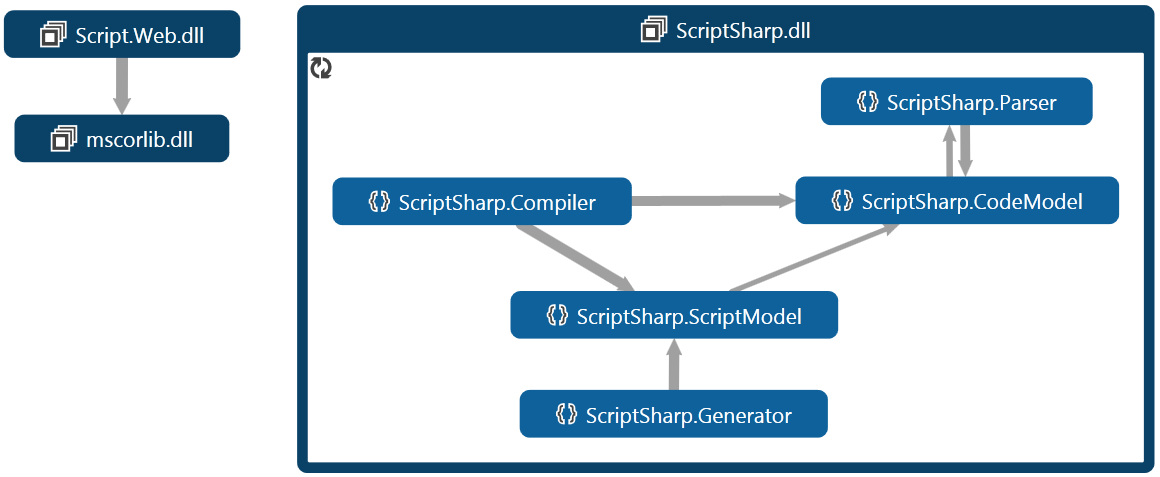
\includegraphics[width=16cm]{resources/images/SimplifiedOverview.png}}
			\end{center}
			\caption{Simplified Script\# architecture overview.}
			\label{simplifiedOverview}
		\end{figure}

		Another important assembly is the Script.Web.dll. This assembly contains classes for Document Object Model (DOM) representation.

		Script\# defines a modified version of the .NET mscorlib.dll so that the (modified) .NET core type interfaces resembles the equivalent JavaScript objects. E.g.\ the Script\# defined System.String type has a CharAt(int index) function that doesn't exist on the original .NET System.String type but that does exist on a JavaScript string object. One benefit of the modified mscorlib.dll is that it makes the C\# compiler able to validate the C\# code that represents JavaScript code entirely (todo: REF to explanation). 

		The modified mscorlib.dll file is referenced in one's Visual Studio project (instead of the original one) when a new ScriptSharp project is created. When a ScriptSharp project is compiled a JavaScript file will be generated. This JavaScript file can then be used in other projects (E.g. a Web Forms web application).
	% subsection subsection_name (end)

	\subsection{Microsoft Roslyn} % (fold)
\label{sub:microsoft_roslyn}
	Roslyn is a Microsoft project that exposes the C\# compiler as a service. There are three key features that makes Roslyn interesting.

	First of all, with Roslyn it is easy to generate an AST from C\# source code. This is done by using either the \texttt{ParseText} or the \texttt{ParseFile} method on Roslyn's \texttt{SyntaxTree} class. The generated AST consists of nodes of type \texttt{SyntaxNode}, which represent C\# constructs such as declarations, statements and expressions. E.g. an \texttt{if}-statement is represented by an \texttt{IfStatementSyntax} node and a binary expression, such as \texttt{1 + 2}, is represented by a \texttt{BinaryExpressionSyntax} node.

	Secondly, the generated AST can be traversed easily thanks to the fact that Roslyn's internal structure is based on the Visitor Pattern \cite{bib:visitorpattern}. By inheriting from Roslyn's \texttt{SyntaxWalker} class, all \texttt{SyntaxNode}s in a given \texttt{SyntaxTree} can be visited and processed as desired. This is done by overwriting the \texttt{SyntaxWalker}'s default \texttt{Visit}-methods. E.g. to visit an \texttt{IfStatementSyntax} node, the \texttt{SyntaxWalker}'s \texttt{VisitIfStatement}-method has to be overwritten.
	TODO: Maybe the last sentence should be moved to implementation section.

	Lastly, Roslyn can create a Semantic Model for any Syntax Tree. The Semantic Model functions as a refence table that contains information about the syntax nodes in the syntax tree. For example, given an expression, the Semantic Model can determine its resultant type. Given an identifier, the Semantic Model can determine its type. This can be very useful, e.g. as many local variables across the source code can have the same name, but different types. So while the SyntaxTree defines the programs syntactic structure, the Semantic Model helps identifying what is being referenced. The Semantic Model is not limited to looking up types defined within the Syntax Tree. If external assemblies (such as mscorlib.dll) is handed to the Semantic Model upon creation, references to types within these assemblies can also be resolved.


% subsection microsoft_roslyn (end)

	% \subsection{Microsoft Roslyn} % (fold)
	% \label{ssub:microsoft_roslyn}

	% % subsection microsoft_roslyn (end)

	\subsection{Code Quotations} % (fold)
	\label{ssub:code_quotations}
		todo
	% subsection code_quotations (end)

	\subsection{Expression Trees} % (fold)
	\label{ssub:expression_trees}
		todo
	% subsection expression_trees (end)

	\subsection{Internal DSL} % (fold)
	\label{ssub:internal_dsl}
		todo
	% subsection internal_dsl (end)

\section{Stages when going from .NET Language to JavaScript} % (fold)
\label{sec:stages_when_going_from_net_language_to_javascript}
	Before discussing different approaches it make sense to clarify the possible stages in the process of ``going'' from a .NET language to the target language. The process (displayed in figure \ref{stages}) moves from left to right and possibly skips stages on the way.

				\begin{figure}[H]
			\begin{center}
				\centerline{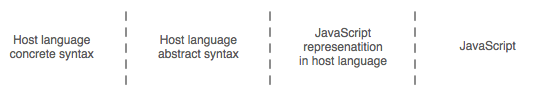
\includegraphics[width=14cm]{resources/images/stages.png}}
			\end{center}
			\caption{Possible approach stages}
			\label{stages}
		\end{figure}

	The .NET concrete syntax is what the developer will be utilizing when writing code. From this concrete syntax a .NET abstract syntax tree (hereinafter AST) can be generated. This AST can be traversed in order to map the .NET AST to a JavaScript representation (typically also an AST) in the .NET language. Finally, JavaScript can be generated from the JavaScript AST.
% section stages_when_going_from_net_language_to_javascript (end)

\section{Possible Approaches} % (fold)
\label{sec:possible_approaches}
	todo text

	todo: update figure
					\begin{figure}[H]
			\begin{center}
				\centerline{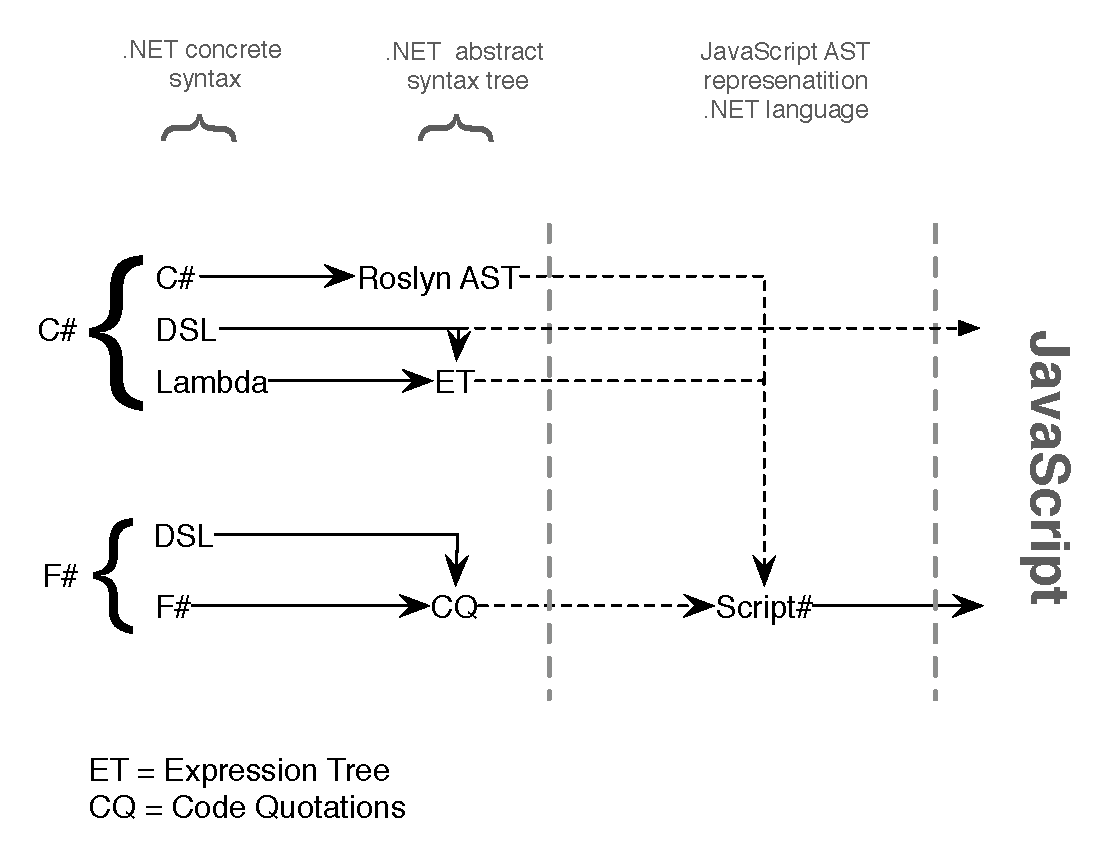
\includegraphics[width=14cm]{resources/images/approachComparison.eps}}
			\end{center}
			\caption{Map of possible approaches. A solid line means that the transition from A to B is given and requires no work on our side. A dashed line means that the transition has to be implemented.}
			\label{approachMap}
		\end{figure}

	\subsection{Internal DSL Approaches} % (fold)
	\label{ssub:internal_dsl_approaches}

		The Internal DSL approaches have been separated into two categories. The first where the DSL is used to build a host language AST which later can be mapped to a target language AST. The second where the target language AST is created directly (i.e.\ the Host Language Abstract Syntax stage is skipped). One significant difference in these two approaches has to do with the possibility of executing code both on server side and client side. When generating the host language AST before mapping to the target language AST its easier to also execute the code in the host language context through dynamic compilation of the host language AST (this approach is discussed in xx TODO).
	
		\subsubsection{Internal DSL Directly to JavaScript AST} % (fold)
		\label{sub:internal_dsl_directly_to_javascript_ast}
		
			When utilizing an internal DSL one would need classes for representing primitive types, expression, statements etc. All the target language features that one will make available needs to be mapped to a DSL representation. Every DSL call would then instantiate an equivalent target language AST node.

			One thing important to consider when creating a DSL representing a different language is its syntax. The DSL syntax should resemble the target language concrete syntax so that the DSL is easily utilized by the target users. At the same time, it should make the verbose instantiation (see example below) of host abstract syntax less cumbersome.

			todo: redo code example

		% subsection internal_dsl_directly_to_javascript_ast (end)

		\subsubsection{C\# DSL} % (fold)
		\label{sub:cs_dsl}

			To approach the project initially we did some experiments with a DSL (in C\#) that created a JavaScript AST directly (i.e. the .NET Abstract Syntax tree stage was skipped) (TODO: See appendix for class diagram and maybe description of scope / block handling mechanism etc.). Using helper factory methods (to create AST nodes), operator overloading and a scope and block handling mechanism (utilizing Statement Lambdas) one can arrive at a DSL syntax that could be somewhat compared to concrete syntax (see example below).

			todo: redo code example

			However, there are different problems with this approach. First of all the syntax doesn't exactly resemble regular C\# or JavaScript. This implies that there will be a learning effort before the DSL can be used. Furthermore the syntax is a bit verbose and readability is also decreased a bit.

			Another problem with the C\# DSL implementation is that the initial declaration and assignment of the variable ``i'' is done using ``='' operator where any subsequent assignments should be done using the ``Assign(...)'' method (or possibly through overloading an existing operator e.g. \texttt{\%=}). The main reason for this is that it is not possible to override the assignment operator in C\# (QUOTATION). This is a critical problem because if the regular C\# assignment operator, \texttt{=}, was used incorrectly by mistake it would not trigger any exceptions and therefore cause a difficult to debug error.  The example below shows exactly this. The variable ``i'' is assigned in an incorrect manner after its initial declaration according to the DSL syntax.

			todo: redo code example
		
		% subsection subsection_name (end)

		\subsubsection{F\# DSL} % (fold)
		\label{sub:fs_dsl}

			The problem with not being able to overload the assignment operator (illustrated in figure todo: REF) would not be an issue in F\# as the assignment operator could be overloaded. Furthermore it is even possible to implement new operators consisting of one or more characters from a given set of characters, consequently making it possible to implement some special JavaScript operators such as strict equal (===).

			One problem though with the F\# DSL approach is the fact that the F\# native syntax and programming paradigm (e.g. the use of immutable types) is radically different from that of JavaScript (and C\# for that matter). This would imply a steep learning curve according to our target user as one would have to learn the F\# syntax and programming paradigm together with the DSL. Even if F\# was the language of choice there would be other powerful language features (i.e.\ Code Quotations) that might bias one toward a different approach (see section \ref{sub:using_fs_code_quotations}).
		% subsection fs_dsl (end)

		\subsubsection{DSL to .NET AST} % (fold)
		\label{sub:dsl_to_net_ast}
			To accommodate server client portability one option in C\# is to utilize Expression Trees. With this approach the DSL would build a .NET AST represented as an Expression Tree which hereafter could be mapped to JavaScript. The .NET AST can also be compiled into host language executable code using the Compile() feature (todo: QUOTATION) on Expression Trees. With an F\# DSL approach a similar pattern could be achieved with Code Quotations (the Expr type). A more straightforward solution to the mixed side execution goal would though be to not use a DSL. Instead one would use the concrete syntax of host language. Then utilize dynamic compilation to retrieve the host language AST which is what we'll discuss in the next section (todo: REF ``Using Roslyn'').
		% subsection dsl_to_host_ast (end)
	% subsubsection internal_dsl_approaches (end)


	\subsection{Host Language Approaches} % (fold)
	\label{sub:host_language_approaches}
		Instead of using an internal DSL, tools (or in some cases language features) exist to generate AST’s from native host language code. These can be traversed and processed as desired by the programmer.

		As tools handle the generation of a host language AST, the workload imposed on the programmer by using this approach is considerably smaller than using e.g. an internal DSL. When using an internal DSL it is up to the programmer to implement a library that represents its concrete syntax.

		The workload is also lightened on the developer. When using tools to generate a host language AST it is possible for the developer to write native code and have it converted to JavaScript instead of having to learn how to use a new library.

		As the host language AST is generated from native host language code it is possible to use the same code on both client side and server side, as the client side code is generated from the server side code. This is very useful with cases such as form validation as it is not necessary for the developer to write the same logic in two different languages. Furthermore, it allows the developer to generate client side code reusing code from previous C\# projects.

		Another benefit of using native host language code, is the possibility of testing on server side. As the code is able to run and evaluate on server side, the developer won't have to write tests in two different languages as the unit testing framework has effectively also been applied to the client side code.

		One disadvantage of using an AST generated from a native host language is that there are no restrictions on what the developer might do. The scope of the project is set by our case study, and as such, our solution will be unable to convert every single construct of an entire language. Should the developer choose to use a language construct that our solution does not support, it will result in a (server-side) runtime error, whereas a DSL would already discover this on compile time. The reason for this is the intrinsic limiting nature of a DSL (todo: REF BOOK: Domain Specific Languages + clarify intrinsic limited nature).

		\subsection{Using F\# Code Quotations} % (fold)
		\label{sub:using_fs_code_quotations}
		
			Code Quotations is a built-in feature in the F\# language which lets a developer generate an abstract syntax tree that represents the corresponding F\# code. Code Quotations cover the entire F\# language, meaning that theoretically all F\# constructs can be mapped to a corresponding JavaScript construct.

			The main disadvantage of using Code Quotations is that they require the end user to know a different language from the one in which ASP.NET WebForms Applications are typically written (C\#). This would probably not be a very great barrier if the syntax of the language didn't vary as much as F\# does from C\#. Also, C\# and JavaScript are somewhat similar in syntax, whereas F\#'s and JavaScripts syntaxes are beyond comparison.
		% subsection using_f#_code_quotations (end)

		\subsection{Using C\# Expression Trees} % (fold)
		\label{sub:using_cs_expression_trees}
			Expression Trees is a built-in feature in the C\# (and Visual Basic) language that “represents code in a tree-like data structure, where each node is an expression, for example, a method call or a binary operation” (REF MSDN). Expression Trees are often used with LINQ to build dynamic queries, which can be useful when fetching data from a database with filters specified by the user (these filters may be provided through a user interface). Expression Trees can be generated from lambda expressions, and thus it is possible to retrieve a representation of simple pieces of code, such as the following:

			todo: code example: Func<int, int, bool> function = (a, b) => a > b

			or more sophisticated ones such as LINQ queries.  A major pitfall using Expression Trees is that they cannot be generated from lambda statements, which prevents the possibility of generating AST’s from blocks of code.
		% subsection using_C\#_expression_trees (end)

		\subsection{Using Roslyn} % (fold)
		\label{sub:using_roslyn}
			Roslyn is a Microsoft project that exposes the C\# and Visual Basic compilers as services. Even though the two are alike, we will focus on C\#. As with F\# Code Quotations, Roslyn is able to generate an AST from C\# source code, and as with Code Quotations, Roslyn is full fidelity (REF) which means that all C\# constructs can be recognized and parsed into syntax nodes. In fact, the AST generated by Roslyn contains every single character of the original source code, down to the last piece of whitespace. Thus, Roslyn combines the advantages of Code Quotations and Expression Trees by allowing the generation of an AST from every C\# construct (including blocks), and avoiding the unfamiliar F\# syntax.
		% subsection using_roslyn (end)
	% subsection host_language_approaches (end)

% section possible_approaches (end)

\section{Deciding on Approach} % (fold)
\label{sec:deciding_on_approach}
	todo: text

						\begin{figure}[H]
			\begin{center}
				\centerline{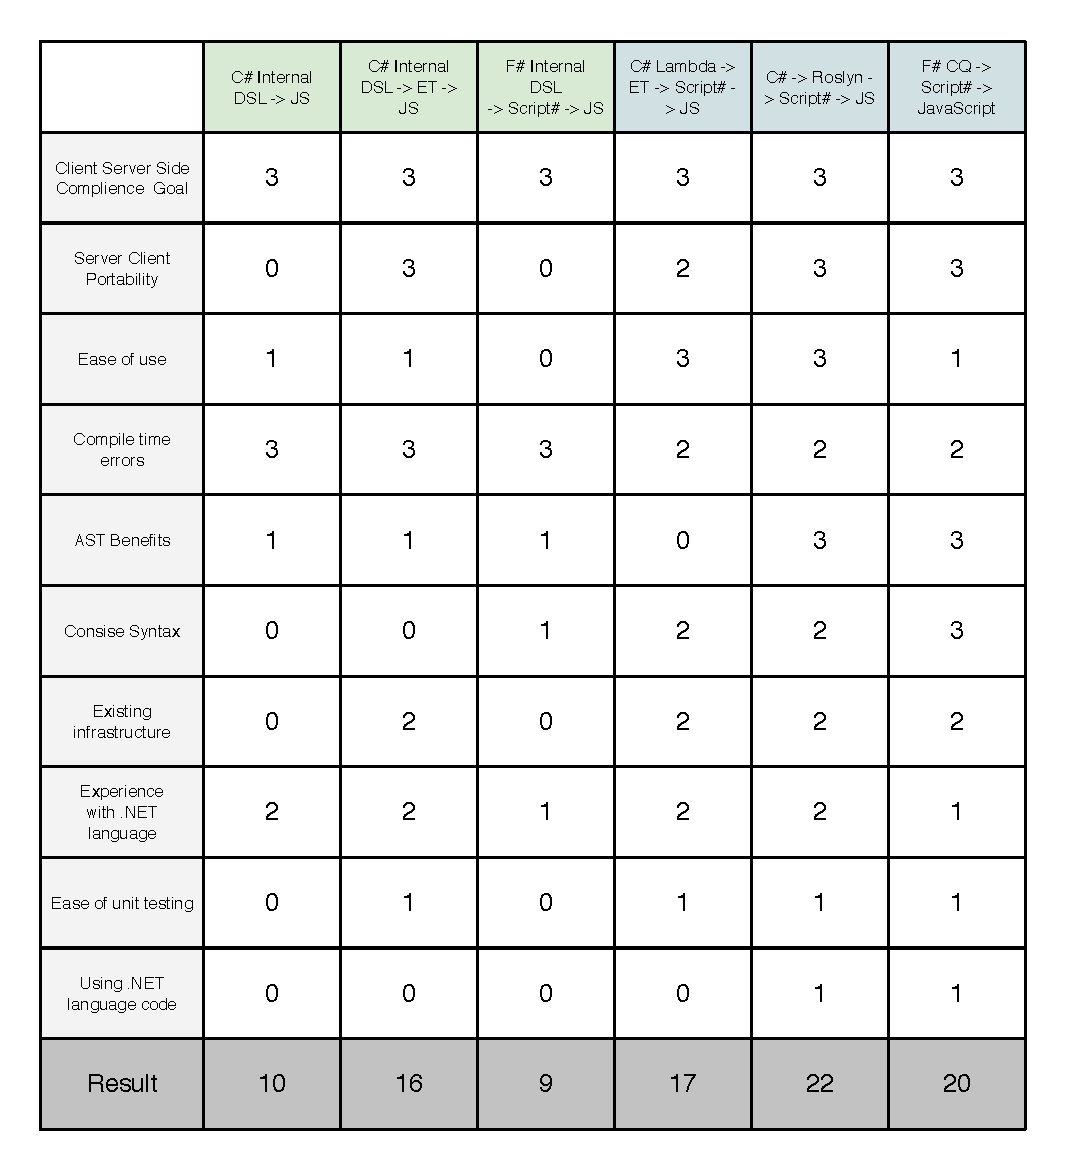
\includegraphics[width=16cm]{resources/images/approachmatrix.eps}}
			\end{center}
			\caption{Approach Matrix.}
			\label{approachMatrix}
		\end{figure}


	todo: shorter column titles on approach matrix + concluding text

	\subsection{Detailed Scope} % (fold)
	\label{sub:detailed_scope}
	
	% subsection detailed_scope (end)
% section deciding_on_approach (end)
\chapter{MiCS User Manual}
\label{chap:mics_manual}
MiCS is a framework that makes it possible to write JavaScript safely by translating C\# to JavaScript. This approach also makes it possible to execute the same code both on server and client side and it ensures consistency between JavaScript code and Html elements.

This chapter demonstrates how to use MiCS. The manual will illustrate how to write server side code that can be reused on client side in a safe manner. It is assumed that the developer uses Visual Studio and .NET 4.0. In this manual a simple registration form, shown in figure \ref{fig:manual_registrationform}, is created. The code is explained step-by-step but can also be found in its entirety in Appendix X (TODO REF).

% Todo: Insert appendix

\begin{figure}[H]
	\begin{center}
		\centerline{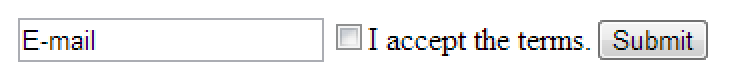
\includegraphics[width=12cm]{resources/images/manual_registrationform.png}}
	\end{center}
	\caption{Simple e-mail registration form.}
	\label{fig:manual_registrationform}
\end{figure}


\subsubsection{1. MiCS-enable Your Web Application} % (fold)
\label{ssub:mics_enable_your_web_application}
Create a new ASP.NET Web Application and add a reference to the MiCS.dll. Goto the \texttt{Default.aspx.cs} Code Behind file and add using statements for \texttt{System.Html}, which contains all the ClientSide DOM types and \texttt{MiCS}. Change the \texttt{Default} class to inherit from \texttt{MiCSPage} instead of \texttt{System.Web.UI.Page}. See figure \ref{fig:mics_enable_web_application}.
\begin{figure}[H]
\begin{lstlisting}[language=CSharp,classoffset=1,morekeywords={Default,MiCSPage,Button,CheckBox,TextBox,EventArgs,ClientSide,InputElement,Document,CheckBoxElement,Window,MixedSide,Regex}]
...
using MiCS;
using System.Html;

namespace MiCSManual
{
    public partial class Default : MiCSPage
    {
        protected void Page_Load(object sender, EventArgs e)
        {
   
        }
    }
}
\end{lstlisting}
\caption{MiCS enabled Default.aspx.cs Code Behind file}
\label{fig:mics_enable_web_application}
\end{figure}
% subsubsection mics_enable_your_web_application (end)

Add the relevant controls to the page, as shown in figure \ref{fig:mics_add_controls}

\begin{figure}[H]
\begin{lstlisting}[language=CSharp,classoffset=1,morekeywords={Default,MiCSPage,Button,CheckBox,TextBox,EventArgs,ClientSide,InputElement,Document,CheckBoxElement,Window,MixedSide,Regex}]
...

public partial class Default : MiCSPage
{
  Button button;
  CheckBox checkBox;
  TextBox emailBox;

  protected void Page_Load(object sender, EventArgs e)
  {
    emailBox = new TextBox() { ID = "EmailBox", Text = "E-mail" };
    checkBox = new CheckBox() { ID = "CheckBox", Text = "I accept the terms."};
    button = new Button() { Text = "Submit" };

    form1.Controls.Add(emailBox);
    form1.Controls.Add(checkBox);
    form1.Controls.Add(button);
  }
}

...
\end{lstlisting}
\caption{Add simple registration form controls from Code Behind}
\label{fig:mics_add_controls}
\end{figure}
% subsubsection mics_enable_your_web_application (end)



\subsubsection{2. Writing MiCS Code} % (fold)
\label{ssub:writing_mics_code}
It is now possible to write code that can be used both on server side and client side. This can be done by adding the MixedSide attribute to a method, as shown in figure \ref{fig:write_mics_code}

\begin{figure}[H]
\begin{lstlisting}[language=CSharp,classoffset=1,morekeywords={Default,MiCSPage,Button,CheckBox,TextBox,EventArgs,ClientSide,InputElement,Document,CheckBoxElement,Window,MixedSide,Regex}]
...
using System.Text.RegularExpressions;

namespace MiCSManual
{    
  public partial class Default : MiCSPage
  {
    ...

    [MixedSide]
    bool IsEmailValid(string email)
    {
      var emailRegex = new Regex("^[A-z0-9._%+-]+@[A-z0-9.-]+.[A-z]{2,4}$");
      return emailRegex.IsMatch(email);
    }
  }
}
\end{lstlisting}
\caption{E-mail validation function that can be used both on server and client side.}
\label{fig:write_mics_code}
\end{figure}

Code that is only intended for use on client side only, can be written in a similar manner, but by adding the \texttt{ClientSide} attribute to the method. In figure \ref{fig:write_mics_code_clienside} a button click event handler has been created. The method is supposed to run on client side when the submit button is clicked. Notice how the method makes use of the \texttt{MixedSide} isEmailValid method.


\begin{figure}[H]
\begin{lstlisting}[language=CSharp,classoffset=1,morekeywords={Default,MiCSPage,Button,CheckBox,TextBox,EventArgs,ClientSide,InputElement,Document,CheckBoxElement,Window,MixedSide,Regex}]
[ClientSide]
bool button_ClientClick()
{
  var emailField = (InputElement)Document.GetElementById("EmailBox");
  var termsCheckBox = (CheckBoxElement)Document.GetElementById("CheckBox");
  
  if (!isEmailValid(emailField.Value))
  {
    Window.Alert("Invalid E-mail!");
    return false;
  }
  
  if (!termsCheckBox.Checked)
  {
    Window.Alert("Accepting terms are required!");
    return false;
  }
  
  return true;
}
\end{lstlisting}
\caption{Client side only method that calls the \texttt{IsEmailValid} mixed side method. Both methods resides on the \texttt{Default} class.}
\label{fig:write_mics_code_clienside}
\end{figure}
% subsubsection writing_mics_code (end)

\subsubsection{3. Register Click Events} % (fold)
\label{ssub:3_register_click_events}
	The last thing that needs to be done is registering click events on the submit button, both for the client and server side. Web Controls like buttons also have server side events in ASP.NET Web Forms. Registering click events is done as the last thing in the \texttt{Page\_Load} event as shown in figure \ref{fig:register_events}. Note that the server side click event handler is also defined here.
\begin{figure}[H]
\begin{lstlisting}[language=CSharp,classoffset=1,morekeywords={Default,MiCSPage,Button,CheckBox,TextBox,EventArgs,ClientSide,InputElement,Document,CheckBoxElement,Window,MixedSide,Regex}]
protected void Page_Load(object sender, EventArgs e)
{
  ...

  // Register the server side click event
  button.Click += button_Click;

  // Register the client side click event
  button.OnClientClick(button_ClientClick);
}

void button_Click(object sender, EventArgs e)
{
  if (isEmailValid(emailBox.Text) && checkBox.Checked)
    form1.Controls.Add(new Label() { Text = "Registration Complete." });
  else
    form1.Controls.Add(new Label() { Text = "Server Side Registration Failed!" });
}
...
\end{lstlisting}
\caption{Registration of both server and client side button click events.}
\label{fig:register_events}
\end{figure}

% subsubsection 3_register_click_events (end)

Now the example web application can be run. If the client side validation passes, the form is submitted and validated on server side as well.

If the user does not enter a valid e-mail address or doesn't accept the terms, he will be alerted with an error message and the form will not submit. Should the user bypass the client side validation, the server side validation will step in, and the user will be met with an error message generated from server side instead.

The resulting HTML and JavaScript source code is shown in Figure \ref{fig:manualHtmlSource}.

\begin{figure}[H]
\begin{lstlisting}[language=html]
<!DOCTYPE html>
<html xmlns="http://www.w3.org/1999/xhtml">
<head><title></title></head>
<body>
    <form method="post" action="./" id="form1">
    ...
    <script type="text/javascript">
    //<![CDATA[
    function MiCSManual$Default() {
    }
    MiCSManual$Default.prototype = {
      button_ClientClick: function() {
        var emailField = document.getElementById('EmailBox');
        var termsCheckBox = document.getElementById('CheckBox');
        if (!this.isEmailValid(emailField.value)) {
          window.alert('Invalid E-mail!');
          return false;
        }
        if (!termsCheckBox.checked) {
          window.alert('Accepting terms are required!');
          return false;
        }
        return true;
      },
      isEmailValid: function(email) {
        var emailRegex = new RegExp('^[A-z0-9._%+-]+@[A-z0-9.-]+.[A-z]{2,4}$');
        return emailRegex.test(email);
      }
    };
    //]]>
    </script>
    ...
    <input name="EmailBox" type="text" value="E-mail" id="EmailBox" />
    <input id="CheckBox" type="checkbox" name="CheckBox" />
    <label for="CheckBox">I accept the terms.</label>
    <input type="submit" name="ctl03" value="Submit" 
     onclick="var obj = new MiCSManual$Default(); return obj.button_ClientClick();" />
    </form>
</body>
</html>
\end{lstlisting}
\caption{The manual example's resulting HTML source code.}
\label{fig:manualHtmlSource}
\end{figure}

In this simple registration form example we have now essentially written JavaScript in a safe manner, we have reused code on server and client side and we have ensured consistency between Html and JavaScript by registering the client side click event in a safe (compile time validated) manner.


\chapter{MiCS Design}

\section{Types in MiCS} % (fold)
\label{sec:types_in_mics}
	To help understand the core type validation and MiCS type mapping in general its beneficial to realise the different kind of types that are utilized in MiCS.

	\begin{figure}[H]
		\begin{center}
			\centerline{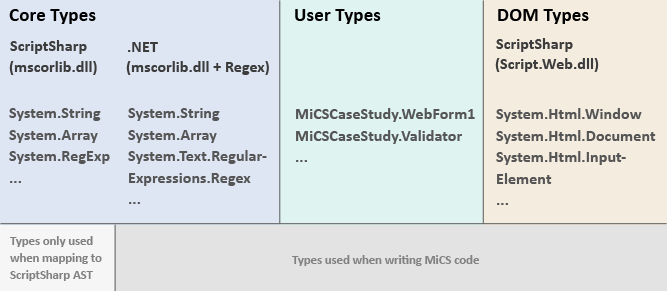
\includegraphics[width=16cm]{resources/images/TypesOverview.png}}
		\end{center}
		\caption{The different types used by MiCS.}
		\label{typesOverview}
	\end{figure}

	Since one of the goals of MiCS is to be able to execute the same code on both client and server side (server client portability) its required that the .NET core types are used when writing MiCS code. This is in contrast to how Script\# works in its original manner where the Script\# core types (that reflect the equivalent JavaScript types) are used. This has some benefits but is also an obstacle that prevents server client portability.

	\subsection{Core Types} % (fold)
	\label{sub:core_types}
		To build the ScriptSharp AST correctly the ScriptSharp core types are required to be associated to the AST nodes. One reason the ScriptSharp core types are required is that they define their equivalent script name (in the class attributes) that is used by the ScriptSharp script generator. An example is the System.Char (see figure \ref{char}) type which is converted to the JavaScript String type as no JavaScript Char type exists.

	\begin{figure}[H]
			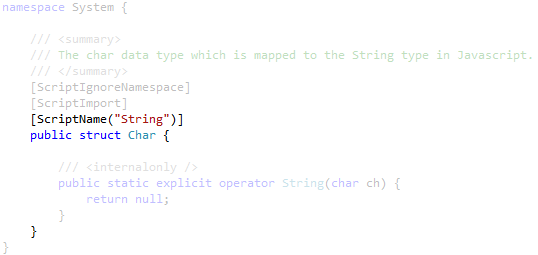
\includegraphics[width=13cm]{resources/images/Char.png}
		\caption{The core type System.Char defined in the Script\# mscorlib.dll.}
		\label{char}
	\end{figure}

		MiCS uses the regular .NET core types when a developer is writing MiCS code but when generating the client side script the Script\# defined core types are used. This implies that some kind of mapping between the two kinds of core types are required. This mapping of core types is explained in section \ref{sub:type_mapping}.
	% subsection core_types (end)

	\subsection{User Types} % (fold)
	\label{sub:user_types}
		User types are the types that are defined by the developer. The user types considered here are either MixedSide types or ClientSide types (i.e. types that have method members that have the either the MixedSide attribute or the ClientSide attribute on them). User type definitions is what the generated client side script eventually will consist of. 

		Pure server side types are obviously also user types but they are not relevant in a MiCS context as JavaScript will not be generated from them.
	% subsection user_types (end)

	\subsection{DOM Types} % (fold)
	\label{sub:dom_types}
		Document Object Model (DOM) types are Script\# infrastructure defined in the System.Html namespace (Script.Web.dll). These classes that represent DOM objects from the browser. The purpose of these classes is only to represent the interface of the actual DOM types in the browser. This is also seen if one looks at the implementation of these types as all their methods and properties on these types return null or false. Like the Script\# core types, DOM types also has their script names in the attribute [ScriptName]. The DOM types are only meant for ClientSide code.

		\begin{figure}[H]
				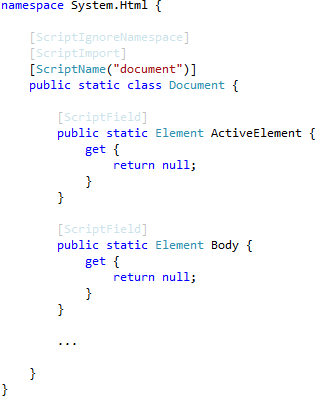
\includegraphics[width=7cm]{resources/images/Document.png}
			\caption{Script\# definition of the DOM type Document.}
			\label{fig:document}
		\end{figure}
	% subsection dom_types (end)

% section types_in_mics (end)

	\section{The MixedSide Principle} % (fold)
	\label{sub:the_mixedside_principle}
		The Mixed Side Principle is a fundamental constraint that the developer has to comply with when using MiCS. In a MiCS web application project there are three kinds of code the user can write; server side code, mixed side code (annotated with the \texttt{MixedSide attribute}) and client side code (annotated with the \texttt{ClientSide} attribute). The Mixed Side Principle describes a simple rule set for the interactions between the different kinds of code. 

		The Mixed Side Principle states that; \emph{Mixed side code can only use other mixed side code. Server and client side code can use mixed side code and code of their own kind respectively.}

		The Mixed Side Principle is illustrated in Figure \ref{fig:MixedSidePrinciple}.

		\begin{figure}[H]
			\begin{center}
				\centerline{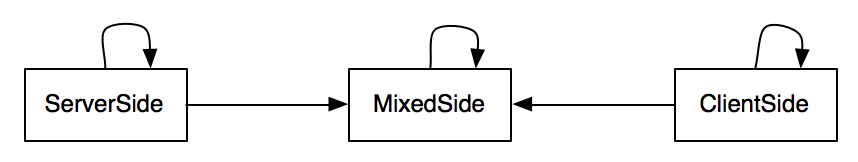
\includegraphics[width=12cm]{resources/images/MixedSidePrinciple.png}}
			\end{center}
			\caption{The Mixed Side Principle. Arrows indicate which kind of code is allowed to be used by the specific kind.}
			\label{fig:MixedSidePrinciple}
		\end{figure}

		Code annotated with the \texttt{ClientSide} attribute is only meant to be run on client side in form of generated JavaScript. Therefore client side code cannot make calls to server side only objects. This would not make sense as server and client side are two different and separated execution contexts.  If client side code were to call server side code, it would ultimately result in a client side error as the server side code will not be mapped to client side. Likewise it will not make sense for server side code to call client side code.

		However mixed side code can be called both from client and server side code. Mixed side code can however only consist of C\# constructs, supported by MiCS, that can be mapped to JavaScript. Mixed side code can only call other mixed side code therefore it cannot use client side only types such as DOM types. This would simply not make sense when mixed side code is called from server side.

		All three kinds of code can obviously use other code of the same kind hence the recursive arrows in illustartion \ref{fig:MixedSidePrinciple}.

\section{Workflow Overview} % (fold)
\label{sec:workflow_overview}

This section provides a brief overview of how MiCS works. Figure \ref{fig:mics_internal_workflow} shows the five stages that MiCS goes through when converting C\# to JavaScript.

Basically, MiCS uses Roslyn to generate an AST representing the user’s C\# code. This AST is validated and mapped to a Script\# AST, that represents JavaScript. From the Script\# AST, JavaScript is generated and finally injected into the user’s WebForm page.

\begin{figure}[H]
	\begin{center}
		\centerline{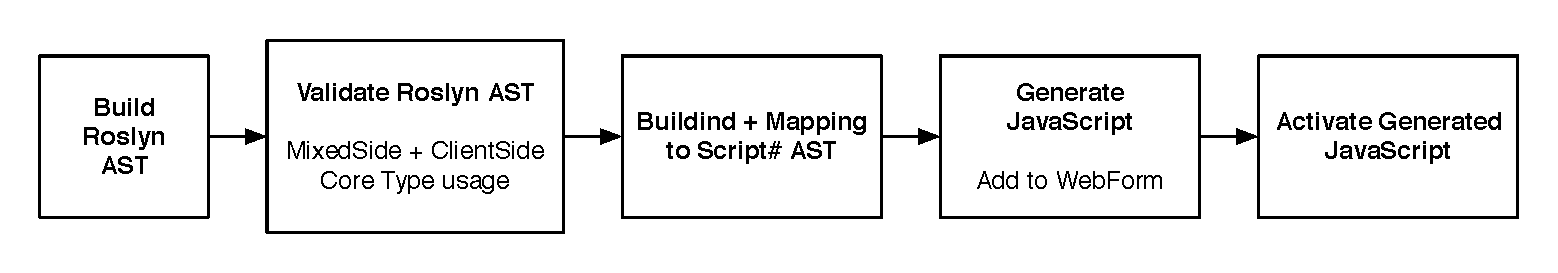
\includegraphics[width=14cm]{resources/images/internalworkflow.eps}}
	\end{center}
	\caption{The MiCS internal workflow}
	\label{fig:mics_internal_workflow}
\end{figure}

MiCS uses Roslyn to generate an Abstract Syntax Tree which is a syntatic representation of the user’s C\# code. Apart from the AST, a Semantic Model is generated to obtain information about what is being referenced.

When the Roslyn AST has been obtained it needs to be validated. This is done to ensure that the user uses types in a correct manner. Without validation, it would be possible for the user to generate non-working JavaScript.

Once the syntax tree has been validated, it is ready to be mapped to Script\#. This is the core functionality of MiCS - transforming a Roslyn AST to a Script\# AST. This step also ensures that the user does not utilize C\# constructs (declarations, statements and expressions) that we do not support. For example, at the moment the only supported loop-type is the for-loop. So if the user uses a while-loop or a foreach loop, the user gets an error telling them that an unsupported construct has been used.

When the Roslyn AST has successfully been mapped to Script\#, MiCS uses Script\#’s built-in ScriptGenerator to generate the JavaScript corresponding to the user’s original C\# code. 

When the JavaScript has been generated, it needs to be injected into the users WebForm. This is handled by a MiCSPage class; an extension to a WebForm Page. 

% section workflow_overview (end)

\section{Architecture} % (fold)
\label{sec:architecture}
Figure \ref{fig:dependencygraph} shows the most essential parts of the internal MiCS architecture and how the parts depend on each other. 
This section will describe the different parts, how they relate to one another and how the architecture relates to the five stages outlined in section \ref{sec:workflow_overview}. 

\begin{figure}
	\begin{center}
		\centerline{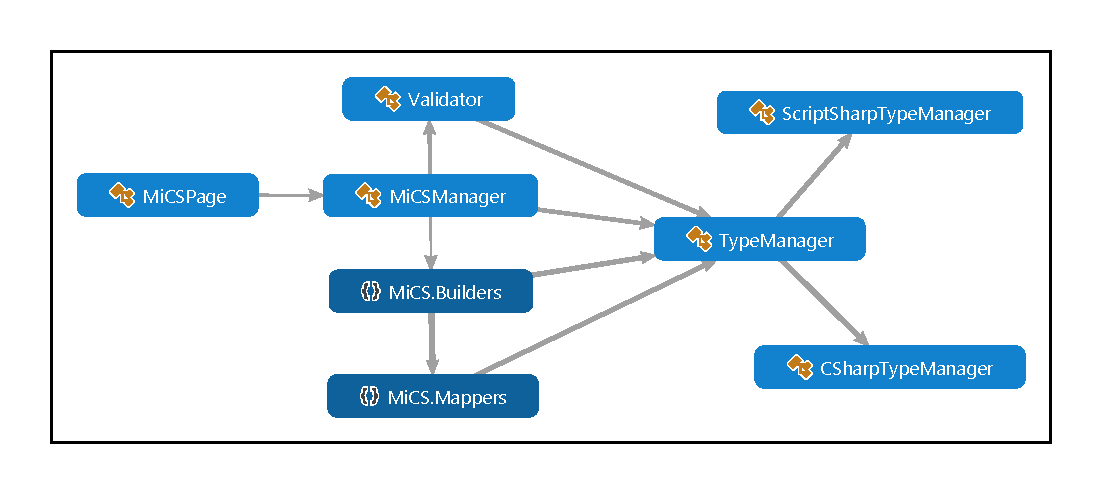
\includegraphics[width=15cm]{resources/images/architecture.pdf}}
	\end{center}
	\caption{The most important parts of the MiCS architecture.}
	\label{fig:dependencygraph}
\end{figure}


The TypeManagers (\texttt{TypeManager}, \texttt{CSharpTypeManager} and\newline \texttt{ScriptSharpTypeManager}) provide information about types used throughout MiCS. For example, the TypeManagers are able to lookup the resultant type of an expression or the type of an identifier (using the Semantic Model described in section \ref{sub:microsoft_roslyn}). Furthermore, they can determine whether a given type is one that the user has defined, or if it is a built-in .NET-type.

The \texttt{Validator} class is responsible for validating the user's code in order to ensure correct type usage before the conversion to Script\# AST begins. The \texttt{Validator} is initiated by the MiCSManager and is dependent on the type managers.

Classes in the Builders and Mappers namespaces are responsible for converting a Roslyn AST to its' corresponding Script\# AST. The Builders traverse the Roslyn AST and build a corresponding Script\# AST. The Builders are dependent on the Mappers which handle the actual conversion from Roslyn SyntaxNodes (AST nodes) to the corresponding Script\# constructs. (Stage 3)

The \texttt{MiCSManager} class ties the entire MiCS project together and is involved in all of the stages described in section \ref{sec:workflow_overview}. It initializes the TypeManagers, starts the validation, and subsequently initiates all of the processes needed to generate JavaScript. 

TODO: Vis og beskriv hvilken del af ScriptSharp vi erstatter med MiCS og Roslyn.
TODO: Update dependency graph

% % section architecture (end)

\section{Usability Considerations}
This section focuses on design considerations conserning usability for the developer. The design considerations mentioned here are mainly nice-to-haves and will not be discussed in the implementation chapter. However, we will reflect upon these considerations in the evaluation.

\subsection{What to generate JavaScript from?} % (fold)
\label{sub:what_to_generate_javascript_from}
	To easily distinguish client side code, mixed side code and server side code from one another, the \texttt{MixedSide} and \texttt{ClientSide} attributes have been introduced. They serve as an easy way for the developer to express which methods that should be used on client side, server side and mixed side respectively. At the same time, they make it easy for MiCS to understand which parts of the developers code to generate JavaScript from. The attributes needs to be used explicit to help ensure that only code intended for client side is actually generated as JavaScript.

% subsection what_to_generate_javascript_from (end)

\subsection{Error messages} % (fold)
\label{sub:design_error_messages}
	As stated in the introduction, it is not our intent to make a complete mapping from C\# to JavaScript. Therefore, when developers use a C\# construct or type that we are unable to map, it is important to fail with an error message that makes sense to the developer. It should not be left to the developer to interpret and debug errors thrown directly from Roslyn. For this reason, different exceptions are implemented. An example of such an exception is the \texttt{MixedSidePrincipleViolatedException} which is thrown, e.g. when code annotated with the \texttt{MixedSide} attribute calls either client or server side code.

	% subsection error_messages (end)

\subsection{Initializing MiCS} % (fold)
\label{sub:initializng_mics}
	There should not be a huge overhead on developers when they want to use MiCS in their projects. In order to acheive this, the process of initializing MiCS has been implemented in the \texttt{MiCSPage} class. When using MiCS, as explained in the user manual (chapter \ref{chap:mics_manual}), the \texttt{MiCSPage} class should be used instead of ASP.NET's \texttt{System.Web.UI.Page} class.
% subsection initializng_mics (end)
\chapter{MiCS Implementation}
	... indledning ...

\section{Types in MiCS} % (fold)
\label{sec:types_in_mics}
	To help understand the core type validation and MiCS type mapping in general its beneficial to realise the different kind of types that are utilized in MiCS.

	\begin{figure}[H]
		\begin{center}
			\centerline{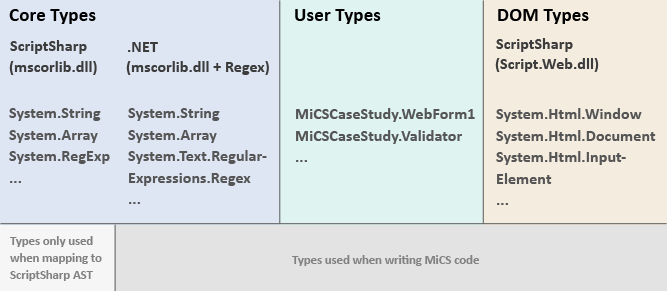
\includegraphics[width=16cm]{resources/images/TypesOverview.png}}
		\end{center}
		\caption{Illustrates the different types used by MiCS.}
		\label{typesOverview}
	\end{figure}

	Since one of the goals of MiCS is to be able to execute the same code on both client and server side (server client portability) its required that the .NET core types are used when writing MiCS code. This is in contrast to how Script\# works in its original manner where the Script\# core types (that reflect the equivalent JavaScript types) are used. This has some benefits but is also an obstacle that prevents server client portability.

	\subsection{Core Types} % (fold)
	\label{sub:core_types}
		To build the ScriptSharp AST correctly the ScriptSharp core types are required to be associated to the AST nodes. One reason why the ScriptSharp core types are required is that they define their equivalent script name (in the class attributes) that is used by the ScriptSharp script generator. An example is the System.Char (see figure \ref{char}) type which is converted to the JavaScript String type as no JavaScript Char type exists.

	\begin{figure}[H]
			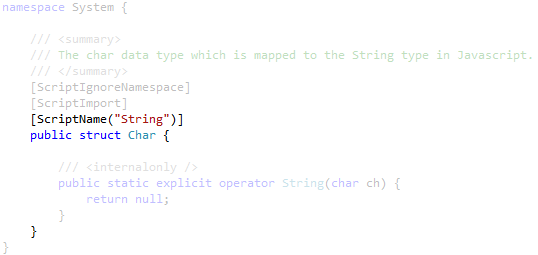
\includegraphics[width=13cm]{resources/images/Char.png}
		\caption{The core type System.Char defined in the Script\# mscorlib.dll.}
		\label{char}
	\end{figure}

		MiCS utilizes the regular .NET core types when a user is writing MiCS code but when generating the client side script the Script\# defined core types are used. This implies that some kind of mapping between the two kinds of core types are required. This mapping of core types is explained in section \ref{sub:type_mapping}.
	% subsection core_types (end)

	\subsection{User Types} % (fold)
	\label{sub:user_types}
		User types are the types that are defined by the MiCS end user. The user types considered here are either MixedSide types or ClientSide types (i.e. types that have method members that have the either the MixedSide attribute or the ClientSide on them). User type definitions is what the generated client side script eventually will consist of. 

		Pure server side types are obviously also user types but they are not that relevant in a MiCS context and therefore not discussed here.
	% subsection user_types (end)

	\subsection{DOM Types} % (fold)
	\label{sub:dom_types}
		Document Object Model (DOM) types are Script\# infrastructure defined in the System.Html namespace (Script.Web.dll). These classes that represent DOM objects from the browser. The purpose of these classes is only to represent the interface of the actual DOM types in the browser. This is also seen if one looks at the implementation of these types as all their methods and properties on these types return null or false. Like the Script\# core types, DOM types also has their script names in the attribute [ScriptName]. The DOM types are only meant for ClientSide code.

		\begin{figure}[H]
				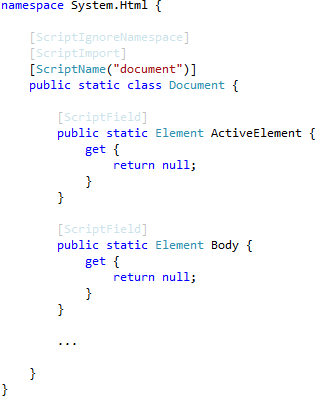
\includegraphics[width=7cm]{resources/images/Document.png}
			\caption{Script\# definition of the DOM type Document.}
			\label{fig:document}
		\end{figure}
	% subsection dom_types (end)

% section types_in_mics (end)

\section{Validating Mixed and Client Side Code} % (fold)
\label{sec:syntax_tree_validation}
	% As we only support a fairly limited set of C\#’s built-in constructs and types, it is important to make sure that users only make use of those that we are able to map to Script\#. Should users utilise one of the constructs or types that we are not able to map, this should be pointed out with an understandable error message. It should not be left to the users to debug or understand a Roslyn or Script\# exception. Furthermore, it is important to make sure that users use their own code correctly. The remainder of this section will describe how a Validator class is used to achieve this.

	Before the Roslyn AST is mapped to Script\# it is necessary to verify that types and their members are used correcly. This is handled by the \texttt{Validator} class. If the developer only uses .NET types that we can map to Script\# and adhere to the Mixed Side Principle, the validation passes. The remainder of this section focus on how this validation is done.
	%Understanding “correct usage of .NET built-in types and members” is straightforward; it means that users are only allowed to use the types and members that can be mapped correctly to Script\#. How this is achieved is described later in this section. However, “correct usage of the types defined by the users themselves” requires some explanation. For this, the MixedSide Principle is introduced.

%To explain correct usage of types and their members, it is beneficial to divide them into two categories; types that are built into the .NET platform and types developers define themselves.



There are essentially three situations in which it is necessary to verify correct usage of types and members.

\begin{itemize}
	\item Object creation; when an instance of a type is created, it is necessary to check the type in question can be mapped.
	\item When members on type instances are accessed; it is then necessary to check first if the type can be mapped, then if the type has a member corresponding to the one being accessed.
	\item Invocation of methods on .NET core types; it is then necessary to check whether the invocation is done correctly, using the correct arguments and return type. Normally, the C\# compiler complains if an invocation is done using an incorrect signature, but as the interface between .NET core types and Script\# core types does not always match, it is important to make sure that the Script\# core type has a member with the corresponding arguments and return type. An invocation that is perfectly legal on .NET core types might be illegal on Script\# core types.
\end{itemize}

The \texttt{Validator} class extends Roslyn's \texttt{SyntaxWalker} class and it is thus able to traverse syntax nodes. The \texttt{Validator} takes a syntax tree that holds the source code to be validated, a string containing an attribute name (''MixedSide'' or ''ClientSide'') that decides what methods to validate, and a structure of types and members that can legally be used without violating the Mixed Side Principle. The \texttt{Validator} works by looking for classes in the syntax tree that contains methods annotated with the given attribute name and validates the body of these methods against the provided structure of allowed members.

The nature of the \texttt{Validator} requires the syntax tree to be validated twice. This is done by creating two instances of the Validator class, a \emph{MixedSide Validator} and a \emph{ClientSide Validator}, and validating them both. 
The MixedSide validator will do \emph{MixedSide validation} and the ClientSide validator will do \emph{ClientSide validation}:

\begin{itemize}
	\item \emph{MixedSide validation} requires validating all the \texttt{MixedSide} methods against a structure containing all \texttt{MixedSide} types and their members
	\item \emph{ClientSide validation} requires validating all the \texttt{ClientSide} methods against a structure containing all \texttt{ClientSide} types and members, \texttt{MixedSide} types and members and Script\# DOM types and members.
\end{itemize}


The Validation process is best explained by looking at an example. Consider a syntax tree holding the simple piece of code shown in figure \ref{fig:mixedSideValidationExample}. The methods of \texttt{ExampleClass} are subjects for MixedSide validation.

\begin{figure}[H]
	\begin{lstlisting}[language=CSharp,classoffset=1,morekeywords={ExampleClass,AnotherExampleClass,MixedSide}]
namespace ExampleNamespace
{
  public class ExampleClass
  {
  	[MixedSide]
  	public void ExampleMethod()
  	{
  		var a = new AnotherExampleClass();
  	}
  }
  
  public class AnotherExampleClass
  {
  	[MixedSide]
  	public void AnotherExampleMethod() { }
  }
}
	\end{lstlisting}
	\caption{Code subject to MixedSide validation}
	\label{fig:mixedSideValidationExample}
\end{figure}		

The MixedSide Validator traverses the syntax tree and discovers the \texttt{ExampleClass} class. It then finds all of the class' methods and checks if they have the \texttt{MixedSide} attribute. When a method annotated with the MixedSide attribute is found, the MixedSide Validator visits it straight away, as shown in Figure \ref{fig:ValidatorVisitClassDeclaration}. 

\begin{figure}[H]
	\begin{lstlisting}[language=CSharp,classoffset=1,morekeywords={ClassDeclarationSyntax,SyntaxKind,MethodDeclarationSyntax,List}]
/// <summary>
/// Visits the ClassDeclaration and determines wether its members should be validated
/// </summary>
public override void VisitClassDeclaration(ClassDeclarationSyntax @class)
{
  List<MethodDeclarationSyntax> methods = @class.DescendantNodes().Where(a => a.Kind == SyntaxKind.MethodDeclaration);
  bool visit = false;

  foreach (var method in methods)
  {
    visit = ((MethodDeclarationSyntax)method).HasAttribute(attributeName);

    if (visit)
      VisitMethodDeclaration((MethodDeclarationSyntax)method);
  }
}
	\end{lstlisting}
	\caption{Visiting a \texttt{ClassDeclarationSyntax} and deciding whether or not its methods should be validated}
	\label{fig:ValidatorVisitClassDeclaration}
\end{figure}


The first method visited is the \texttt{ExampleMethod()} method. The first statement of the method contains an object creation expression and the MixedSide Validator now needs to check if the object creation is legal. It is legal either if the created object is a supported core type, or if the created object is MixedSide type defined by the developer.



As the type exists in the allowed members structure (shown in figure \ref{fig:mixedSideValidationExample}) the object creation is legal and the traversal continues. If it had not existed in the allowed member structure (this could happen if it had been ClientSide), and had not been a supported core type, the MixedSide Principle would have been violated, and an exception of type \texttt{MixedSidePrincipleViolatedException} had been thrown.

The validation of a member access is done in a very similar way, only checking if the member exists in the allowed-members structure or in the core mapping as well.

As mentioned earlier, it is important to validate invocation on core types. This is done using the \texttt{VerifyCorrectUseOfSupportedCoreType} method on the \texttt{TypeManager}. This method first checks if the given invocation is done on a core type, and subsequently uses the Core Mapping Specification (as discussed in section \ref{sub:type_mapping}) to verify that we are able to map the invocation to ScriptSharp.
		



		% When an invocation is visited, the \texttt{TypeManager} is asked to 
		% TODO: Write about how invociations are validated: Only core types need to be validated (with arguments and return types), as user types will automatically be validated by the compiler.


% \begin{lstlisting}[language=CSharp,classoffset=1,morekeywords={TextBox,Panel,CheckBox, Button}]
% TextBox NameBox = new TextBox() { ID = "name", Text = "Name" };
% Panel CheckBoxGroup = new Panel();
% CheckBox SnailMailCheck = new CheckBox() { ID = "dmSnailmail", Text = "Snail Mail" };
% CheckBox EmailCheck = new CheckBox() { ID = "dmEmail", Text = "E-Mail" };
% TextBox AddressBox = new TextBox() { ID = "address", Text = "Address" };
% TextBox ZipcodeBox = new TextBox() { ID = "zipcode", Text = "Zip Code" };
% TextBox EmailBox = new TextBox() { ID = "email", Text = "E-mail" };
% TextBox PhoneBox = new TextBox() { ID = "phone", Text = "Phone" };
% Button SubmitButton = new Button() { Text = "Register" };
% \end{lstlisting}






	
	% subsection validating (end)
% section syntax_tree_validation (end)

\section{Mapping to ScriptSharp AST} % (fold)
\label{sec:mapping_to_scriptsharp_ast}
	When converting the validated Roslyn AST to the ScriptSharp AST we have made a logical division of the process. First the actual mapping from one Roslyn AST node to the equivalent ScriptSharp AST node. Secondly building the ScriptSharp AST from all the mapped nodes. The mapping is discussed in this section. 

	\subsection{Mapping to ScriptSharp Expressions, Statements and Symbols} % (fold)
	\label{sub:subsection_mapping_to_scriptsharp_expressions_statements_and_symbols}
		The mapping of Expressions, Statements and Symbols is implemented in three classes (ExpressionMapper.cs, StatementMapper.cs and SymbolMapper.cs). The three classes are logically divided (and named) after the type of ScriptSharp AST object they map to. 

		\begin{figure}[H]
			\begin{center}
				\centerline{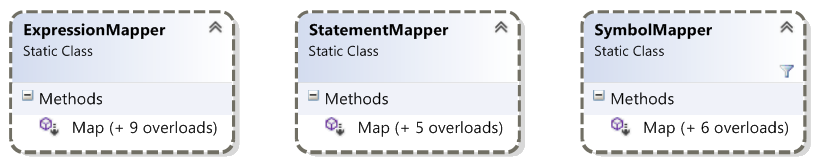
\includegraphics[width=14cm]{resources/images/MapperClasses.png}}
			\end{center}
			\caption{Classes that define extension methods for mapping Roslyn AST nodes to Script\# AST nodes.}
			\label{mapperClasses}
		\end{figure}

		The mapping of the AST nodes is somewhat straightforward as most of the mappings we have done the Roslyn AST maps one to one with the ScriptSharp AST. So a Roslyn return statement node maps to a ScriptSharp return statement etc. The three classes define Map(...) extension methods to the Roslyn objects they map from (see example figures \ref{returnStatementMap} and \ref{conditionaleExpressionMap}).

		\begin{figure}[H]
			\begin{center}
				\centerline{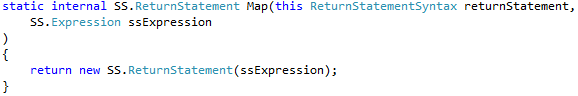
\includegraphics[width=14cm]{resources/images/ReturnStatementMap.png}}
			\end{center}
			\caption{Extension method that maps Roslyn return statement to Script\# return statement.}
			\label{returnStatementMap}
		\end{figure}

		\begin{figure}[H]
			\begin{center}
				\centerline{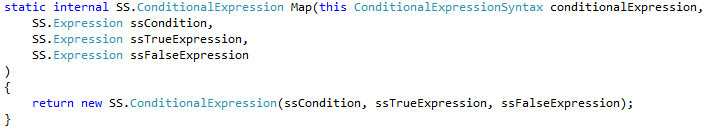
\includegraphics[width=14cm]{resources/images/ConditionalExpressionMap.png}}
			\end{center}
			\caption{Extension method that maps Roslyn conditional expression to Script\# conditional expression.}
			\label{conditionaleExpressionMap}
		\end{figure}
	% subsection subsection_mapping_to_scriptsharp_expressions_statements_and_symbols (end)

	\subsection{Type Mapping} % (fold)
	\label{sub:type_mapping}
		Roslyn type symbols are mapped to Script\# type symbols using the SymbolMapper’s Map(...) extension method created for the Roslyn TypeSymbol. The mapping of TypeSymbols from Roslyn to Script\# can be somewhat confusing since there are the different kinds of types (illustrated in figure \ref{typesOverview}) and there are some special cases (such as null which is mapped to the type Object in JavaScript). To illustrate the functionality of the TypeSymbol Map(...) method we have created the flowchart in figure \ref{typeMappingFlowchart}.

			\begin{figure}
			\begin{center}
					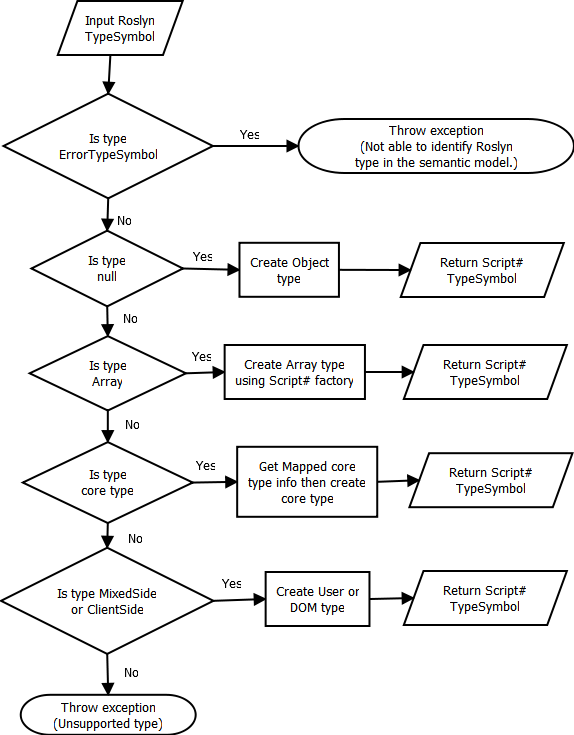
\includegraphics[width=14cm]{resources/images/TypeMappingFlowchart.png}
					\end{center}
				\caption{Illustration of the type mapping process performed in SymbolMapper.Map(this TypeSymbol typeSymbol) extension method.}
				\label{typeMappingFlowchart}
			\end{figure}


		\subsubsection{Core Type Mapping} % (fold)
		\label{subsub:core:type_mapping}
			In contrast to using Script\# in the original manner (where the Script\# core types are used when writing code instead of the .NET core types) our project only uses the Script\# core types when mapping to the Script\# JavaScript AST. For this reason the Script\# core types are handled by its own type manager class (ScriptSharpTypeManager.cs). The Script\# core types’ source code are loaded into their own SemanticModel on the TypeManager class. From here the (Roslyn) types are retrieved before they are mapped to Script\# TypeSymbols needed when building the Script\# AST.

			Since the .NET core types are used when writing MiCS code and since these are mapped to the ScriptSharp core types a mapping specification is needed. To facilitate this mapping we have created some simple classes to hold the specification (MiCSCoreMapping.cs, MiCSCoreTypeMapping.cs and MiCSCoreMemberMapping.cs) which then can queried using LINQ. This mapping specification contains information on the core types that we currently support. So if a core type is not described in the specification then it is not supported. If the core type is found in the specification then the same pattern applies for its members. If a type member is not found then it is not supported. The mapping specification also holds information on a member’s return type, number of arguments and the arguments’ types.

			\begin{figure}[H]
					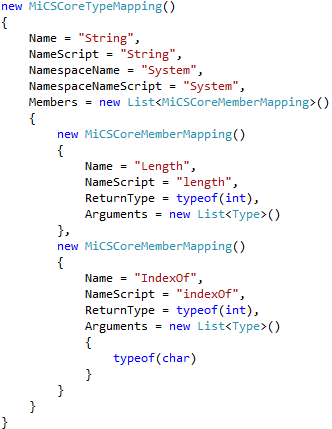
\includegraphics[width=8cm]{resources/images/InitiationOfTypeMapping.png}
				\caption{Instantiation example of a single core type (System.String) mapping specification.}
				\label{coreTypeMapping}
			\end{figure}

			An example of a core type mapping is the C\# System.String (see figure \ref{coreTypeMapping}) type which is mapped to the ScriptSharp defined System.String. We are only mapping two of the String type’s members. The field Length which is mapped to the ScriptSharp String type’s Length field (which is the equivalent of the JavaScript String object property length). The second member we map is the IndexOf(Char char) method that returns an int. There are other IndexOf methods that take multiple arguments or a single argument of a different type (than Char) but these are not mapped in our mapping specification.
		% subsection subsection_name (end)
	% subsection type_mapping (end)
% section mapping_to_scriptsharp_ast (end)

\section{Building the ScriptSharp AST} % (fold)
\label{sec:building_the_scriptsharp_ast}
	Building the Script\# AST consists of taking the mapped (Script\#) AST nodes and putting them together to form the Script\# AST. The builder classes utilize the Roslyn infrastructure by extending the SyntaxWalker class which makes them capable of traversing the Roslyn AST.
	\begin{figure}[H]
		\begin{center}
			\centerline{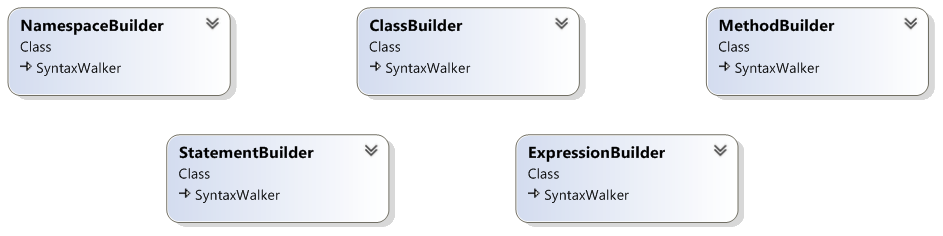
\includegraphics[width=16cm]{resources/images/BuilderClasses.png}}
		\end{center}
		\caption{Classes that built the Script\# AST by traversing the Roslyn AST and utilizing Map(...) extension methods.}
		\label{builderClasses}
	\end{figure}

	The NamespaceBuilder class is responsible for building all of its defined types. This is done by instantiating a ClassBuilder which in turn is responsible for building all of its member methods (which is done by instantiating a MethodBuilder). This implies that the building of the Script\# AST is done in a depth first manner. The NamespaceBuilder and ClassBuilder classes are somewhat trivial. 

	\begin{figure}[H]
		\begin{center}
			\centerline{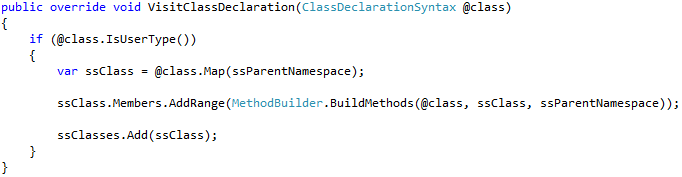
\includegraphics[width=16cm]{resources/images/VisitClassDeclaration.png}}
		\end{center}
		\caption{Empty Script\# class is created and then built by using a MethodBuilder to retrieve all its member methods. The ssClasses property on the builder holds all the classes that will be returned to the NamespaceBuilder who created this class builder.}
		\label{visitClassDeclaration}
	\end{figure}

	The ClassBuilder has an important feature that it ensures that only user defined types will be mapped to the Script\# AST (and generated as script types). DOM (or core) types doesn’t need to be defined in script as these obviously already exists in JavaScript.

	The MethodBuilder class is a little more complex as it needs to only build a method if its a MixedSide or ClientSide method. Furthermore it needs to handle a method’s return type, arguments and body statements. The StatementBuilder and ExpressionBuilder is however the most complex as building compound statements and expressions are more complicated. Before a compound statement or expression can be build all the child nodes and their associated types (if any) needs to be mapped.

	\begin{figure}[H]
		\begin{center}
			\centerline{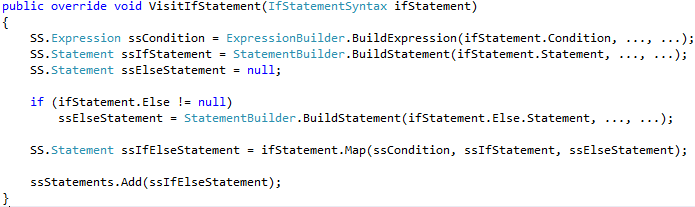
\includegraphics[width=16cm]{resources/images/VisitIfStatement.png}}
		\end{center}
		\caption{To built an IfStatement node its child nodes; condition, if-block and else-block (if any) has to be built first.}
		\label{visitIfStatement}
	\end{figure}

	When a builder class is done building the node(s) are returned to the parent builder class. Once all the namespaces has been built these constitute the Script\# AST which is then passed on in the overall workflow (to script generation).
% section building_the_scriptsharp_ast (end)

\section{Script Generation} % (fold)
\label{sec:script_generation}
	Script generation is done using the ScriptSharp infrastructure only. Specifically the TypeGenerator class located in the ScriptSharp.Generator namespace is utilized for this. The MiCSManager is responsible for instantiating the TypeGenerator and providing it with the ScriptSharp JavaScript AST type nodes (this happens in the MiCSManager.GenerateScriptText method). The ScriptSharp JavaScript AST consists only of the user defined script types.
% section script_generation (end)

\section{Integration with Web Forms} % (fold)
\label{sec:integration_with_web_forms}
	sdsadq qdqw qwd qwd qw 
% section integration_with_web_forms (end)

\chapter{MiCS Testing}
	The testing done in this project can be divided into two categories; MiCS itself and the case study code. Most of our testing is done on MiCS itself. We have used the Visual Studio built-in unit testing framework for all of our tests.
\section{MiCS} % (fold)
\label{sec:mics}
	While implementing MiCS we have also created multiple unit tests located in the \texttt{MiCSTests} project. These tests primarily cover the features that are required by our case study. Because of the time constraints on this project, the quality of the tests are somewhat varying and the real code coverage is not 100\%. However we have still manage to make some tests on core types, DOM types, statements, expressions, symbols and syntax tree validation.

	We have not performed any formal tests on the validity and quality of the Script\# generated scripts. Here we have instead emphasized building a valid Script\# AST and then relied on the existing Script\# infrastructure to work correctly. The reason for this is again the time constraints and the scope of the project.
% section mics (end)
\section{Case Study Testing} % (fold)
\label{sec:user_code_testing}
	Another benefit of using mixed side code is that you also have to write less tests. All mixed side code can be tested with the unit testing framework originally used only for server side. Therefore relying only on a single unit testing framework (instead of one for server side and another for client side) could be possible in some situations.

	To illustrate this possibility we have also created a small unit testing project \texttt{MiCSCaseStudyTests} that tests the validity of our mixed side case study code (specifically the \texttt{Validator} class).

% section user_code_testing (end)
\chapter{Evaluation}

\section{Reflection on Case Study} % (fold)
\label{sec:reflection_on_case_study}
	\begin{itemize}
		\item It's doable. Horray!
		\item Comparison between MiCS and other form validation frameworks (Hvis der er tid)
	\end{itemize}
% section reflection_on_case_study (end)

\section{Ease of Use} % (fold)
\label{sec:ease_of_use}

	\begin{itemize}
		\item Elaborate on the user friendliness of error messages, why they are important
		and to which degree we have implemented them.
		\item Indlæringskurve. Tungen lige i munden. Client-Server confusion
	\end{itemize}
% section ease_of_use (end)

\section{Reflection on Implementation} % (fold)
\label{sec:reflection_on_implementation}
Todo: Skriv noget om at dette afsnit bl.a.\ omhandler forbedringer af den nuværende løsning.

\subsection{Validation} % (fold)
\label{ssub:validation}
It is necessary to make sure that developer only uses C\# constructs (method declarations, various statements and expressions, etc.) that we can correctly map to Script\#. At the moment, this is handled by the Builder classes, and will be explained in a later section. However, optimally this should be the responsibility of the Validator class. How this can be achieved is described in future work.

As explained in section X, at the moment, when validating the Roslyn AST a members structure.
% subsection validation (end)

\subsection{Integration with Web Forms} % (fold)
\label{ssub:integration_with_web_forms}
Todo
% subsection integration_with_web_forms (end)

\subsection{Initializing MiCS} % (fold)
\label{ssub:collecting_source_code}
Todo
% subsection collecting_source_code (end)

\subsection{Extendability} % (fold)
\label{sub:extendability}

% subsection extendability (end)

% section reflection_on_implementation (end)
\section{Reflection on Design} % (fold)
\label{sec:reflection_on_design_goals}
	\begin{itemize}
		\item Mixed Side Code limited to JavaScript enabled features (?)
		\item Runtime vs. Compile Time Errors
		\item Existing code to JavaScript (and testing)
		\item Necissity of MiCS (e.g. JavaScript games would probably use ScriptSharp)
	\end{itemize}

% section reflection_on_design_goals (end)


\section{Safety Benefits vs. Convenience} % (fold)
\label{sec:safety_benefits_vs_conveniente}


% section safety_benefits_vs_conveniente (end)
\section{Future Work}
\begin{itemize}
	\item Inheritance
	\item Portability of Server Side values
\end{itemize}
\chapter{Conclusion}
In this project we have shown how the use of JavaScript can be improved when developing web applications with ASP.NET Web Forms. Especially the three following improvements have been adressed:

\begin{enumerate}
	\item Moving errors from client side to server side
	\item Obtaining Server-Client portability
	\item Obtaining JavaScript-HTML consistency
\end{enumerate}

These improvements have been adressed by implementing the MiCS Framework that lets developers write C\# code and have it translated to JavaScript. MiCS uses a combination of Microsoft's Roslyn and Script\# to do this. 

To address point 1 and 2 from the above list MiCS uses Microsoft's Roslyn to generate an AST representing the developer's code. The AST is traversed and mapped to its corresponding Script\# JavaScript AST. MiCS uses Script\#'s built-in script generator to generate actual JavaScript source code from the Script\# AST. 

In order to obtain JavaScript-HTML consistincy, MiCS defines the \texttt{MiCSPage} class - an extension to the ASP.NET Web Forms framework. This class makes sure that the generated JavaScript is registrered to the developer's page correctly.

The case study introduced in chapter \ref{cha:introduction} has been successfully implemented using the MiCS Framework. Furthermore, shortcomings of the implementation of MiCS has been adressed in the evaluation, and the road map in section \ref{sec:futurework} describes which direction the project should take from here.

% Todo: Move into seperate file
\begin{thebibliography}{9}
\bibitem{lamport94}
  Leslie Lamport,
  \emph{\LaTeX: A Document Preparation System}.
  Addison Wesley, Massachusetts,
  2nd Edition,
  1994.


  \bibitem{msdn01}
  Msdn.com,
  \emph{\LaTeX: Introduction to Windows Forms}.
  http://msdn.microsoft.com/da-dk/library/aa983655(v=vs.71).aspx

  \bibitem{msdn02}
  Msdn.com,
  \emph{\LaTeX: Introduction to ASP.NET and Web Forms}.
  http://msdn.microsoft.com/en-us/library/ms973868.aspx

    \bibitem{scriptsharp}
  ScriptSharp.com,
  \emph{\LaTeX: C\# Productivity with JavaScript Ubiquity!}.
  http://scriptsharp.com

  \bibitem{nikhilk}
  Nikhil Kothari,
  \emph{\LaTeX: Nikhil Kothari blog}.
  http://www.nikhilk.net, https://github.com/nikhilk
  
  \bibitem{bib:visitorpattern}
  OODesign.com,
  \emph{Visitor Pattern}
  http://www.oodesign.com/visitor-pattern.html

  \bibitem{bib:wiki_javascript}
  Wikipedia,
  \emph{JavaScript}
  http://en.wikipedia.org/wiki/JavaScript
\end{thebibliography}












\end{document}

% Todo: search for all 'ScriptSharp' instances and replace with 'Script#'
% Todo: check that texttt is used consistently through out the report
% Todo: search and replace e.g. with e.g.\
% Todo: Explain that ScriptSharpTypeManager and CSharpTypeManager holds a semantic model each
% Todo: Explain the different criteria in the approach matrix
% Todo: scope: doesn't look at performance
% Todo: Search and replace ` with '
